\chapter{Spectral Distortions}
\label{chap:SpectralDistortions}
As the \emph{CMB} is composed by photons, it is reasonable to think that it should be described as some black body radiation. Indeed, the measurements from COBE/FIRAS satellite \cite{COBE1996} showed that the CMB spectrum is very compatible with this assumption.\\
However, many physical processes could affect the spectrum of the CMB generating some \textbf{spectral distortions} that were not detectable by the previous experiments.

In the next sections we will discuss the theory of spectral distortions and the physical processes that could generate them. Our goal is to describe how the dissipation of the primordial perturbation generates distortions. 
\section{The thermalization problem}\label{sec:ThermalizationProblem}
The CMB, nowadays, is the relic of the primordial plasma photon component that, at early times, filled the universe. The spectrum that we observe today is influenced by the interactions that occurred between the components of the plasma. For example, several processes can inject energy that then, through scatterings, will be redistributed in the plasma, recovering equilibrium. The problem of determining how equilibrium is reached is usually referred as the \textbf{thermalization problem}. 

To predict the final spectrum of the CMB, we need to understand how these interactions influenced the evolution of the phase space of the photons: as we already know, this is accomplished by the \textbf{Boltzmann equation}.\\ 
In the early universe, photons are mainly subject to scattering processes with electrons and light nuclei (Hydrogen and Helium). To describe these process it is useful to introduce the \emph{dimensionless frequency}
\begin{equation}\label{eq:dimensionless_frequency}
    x\defeq\frac{\nu}{k_BT_z},\qquad T_z\defeq T_0(1+z),
\end{equation}
where $T_0$ is the present temperature of photons and $T_z$ is the temperature that would have a gas of decoupled photons at redshift $z$. In this way $x$ is a \emph{time invariant variable}, since the redshift $\nu=\nu_0(1+z)$ cancels the time dependence of the temperature $T_z$, leaving only the today observed frequency and temperature. The use of this variable strongly simplifies the Boltzmann equation. Indeed, neglecting perturbations, the phase space distribution function is just a function of time and energy only. We can then use $x$ as a measure of the energy of photons, since it is related to their frequency, so that the time independence of $x$ allows to remove the momentum derivatives from the Liouville operator $$ \hat{L}[f]=\frac{df(t,x)}{dt}=\frac{\partial f}{\partial t}+\frac{dx}{dt}\frac{\partial f}{\partial x}=\frac{\partial f}{\partial t}=C[f].$$
Note that in this way, the phase space distribution is stationary if and only if the collision term vanishes. Physically this means that only scatterings can change the number of photons or their energies.

There are three main types of these interactions.
\begin{enumerate}
    \item \textbf{Compton scattering}: this is the main actor in the thermalization of the CMB. In this process photons are scattered by electrons 
    \begin{multicols}{2}
        $$e^{-}(p)+\gamma(k)\rightleftharpoons e^{-}(p')+\gamma(k').$$\vspace{4cm}
        
        \begin{tikzpicture}[>=Latex, scale=1]

        % Incoming electron
        \draw[thick,->-=.6] (-2,-1) -- (0,0) node[at start, above left] {$e^-$} node [midway, above left] {$p$};

        % Incoming photon
        \draw[decorate,decoration={snake}] (-2,2) -- (0,0) node[at start, below left] {$\gamma$} node [midway, above right] {$k$};

        % Scattering vertex
        \filldraw (0,0) circle (2pt);

        % Outgoing electron
        \draw[thick,->-=.6] (0,0) -- (2,-1) node[at end, above right] {$e^-$} node [midway, above right] {$p'$};

        % Outgoing photon
        \draw[decorate,decoration={snake}] (0,0) -- (2,2) node[at end, below right] {$\gamma$} node [midway, above left] {$k'$};
        \end{tikzpicture}
    \end{multicols}
    Each collision results in a transfer of energy between the photon and electron components of the plasma without changing the number of both. The collision term associated with this process is the \textbf{Kompaneets equation}, which reads
    \begin{equation}
        C[f]\bigg|_{CS}=n_e\sigma_T\frac{k_BT_e}{m_e}x^{-2}\frac{\partial}{\partial x}\bigg[x^4\bigg(\frac{\partial f}{\partial x}+\frac{T_z}{T_e}f(1+f)\bigg)\bigg],\label{eq:C_compton}
    \end{equation}
    where $n_e$ is the number of electrons per unit volume, $\sigma_T$ the Thompson cross section and $T_e$ is the temperature of the electrons. \\
    The first term of the equation \eqref{eq:C_compton} account for the \emph{Doppler effect} due to relative motions of the species in the plasma, while the second term describes the \emph{recoil effect} and \emph{stimulated recoil}.
    \item \textbf{Bremsstrahlung}: this phenomenon arises when, during Coulomb scattering between electrons and ions ($H^+$ of charge $Ze$), an extra photon is produced
    \begin{multicols}{2}
        $$e^{-}(p)+H^+(h)\rightleftharpoons e^{-}(p')+H^+(h)+\gamma(k),$$\vspace{4cm}\\
        \begin{tikzpicture}[>=Latex, scale=1]
        % Incoming electron
        \draw[thick,->-=.6] (-2.5,-2) -- (0,0) node[at start, above left] {$e^-$} node [midway, above left] {$p$};

        % Incoming photon
        \draw[thick, dashed, ->-=.6] (-2.5,2) -- (0,0) node[at start, below left] {$H^+$} node [midway, above right] {$h$};

        % Scattering vertex
        \filldraw (0,0) circle (2pt);

        % Outgoing electron
        \draw[thick,->-=.6] (0,0) -- (1.5,-2) node[at end, above right] {$e^-$} node [midway, above right] {$p'$};

        % Outgoing photon
        \draw[thick, dashed, ->-=.6] (0,0) -- (1.5,2) node[at end, below right] {$H^+$} node [midway, above left] {$h'$};

        \draw[decorate,decoration={snake}] (0,0) -- (2,0) node[at end, right] {$\gamma$} node [midway, above] {$k$};
        \end{tikzpicture}
    \end{multicols}
    Note that this process, while transferring energy between different components of the plasma, generates new photons. The corresponding collision term reads
    \begin{align}\label{eq:C_Bremsstrahlung}
        C[f]\bigg|_{BR}&=n_e\sigma_T\frac{K_{BR }\ e^{-x_e}}{x^3_e}[1-f(e^{x_e}-1)],\\
        \nonumber K_{BR}&\defeq\frac{\alpha}{2\pi}\frac{\lambda_e^3}{\sqrt{6\pi}\theta_e^{7/2}}\sum_iZ_i^2n_i\bar g_{ff}.
    \end{align}
    In the above we used the \emph{dimensionless electron frequency} $x_e=\nu/(k_BT_e)$, the \emph{dimensionless electron temperature} $\theta_e\defeq k_BT_e/m_e$ and the \emph{fine structure constant} $\alpha=e^2/(4\pi)\approx\/137$. We are also accounting for the possibility of having different gasses of ions, each with a number of ions per unit volume corresponding to $n_i$. Lastly, we used the electron Compton wavelength $\lambda_e=1/m_e\approx2.43\times10^{-10}$ cm and the \emph{thermally averaged Gaunt factor} $$\bar g_{ff}\approx\begin{cases}
        \frac{\sqrt3}{\pi}\log\frac{2.25}{x_e},\qquad\text{for }x_e\leq0.37,\\
        1\qquad\qquad\quad\ \ \ \ \text{otherwise.}
    \end{cases} $$
    \item \textbf{Double Compton scattering}: this process consists of a regular Compton scattering followed by the emission of a second photon by the scattered electron 
    \begin{multicols}{2}
        $$e^{-}(p)+\gamma(k)\rightleftharpoons e^{-}(p')+\gamma(k_1)+\gamma(k_2).$$\vspace{4cm}

        \begin{tikzpicture}[>=Latex, scale=1]

        % Incoming electron
        \draw[thick,->-=.6] (-2,-1) -- (0,0) node[at start, above left] {$e^-$} node [midway, above left] {$p$};

        % Incoming photon
        \draw[decorate,decoration={snake}] (-2,1) -- (0,0) node[at start, below left] {$\gamma$} node [midway, above right] {$k$};

        % Scattering vertex
        \filldraw (0,0) circle (2pt);

        % Outgoing electron
        \draw[thick,->-=.3, ->-=.8] (0,0) -- (4,-1) node[at end, above right] {$e^-$} node at (3,-.75) [ below left] {$p'$};

        % Outgoing photon
        \draw[decorate,decoration={snake}] (0,0) -- (2,1.5) node[at end, below right] {$\gamma$} node [midway, above left] {$k_1$};
        \draw[decorate,decoration={snake}] (2,-0.5) -- (4,1.5) node[at end, below right] {$\gamma$} node [midway, below right] {$k_2$};
        \end{tikzpicture}
    \end{multicols}
    Assuming that $\gamma(k_2)$ is a soft photon, namely $k_2\ll m_e$, the collision term for this interaction reads
    \begin{align}\label{eq:C_DCS}
        C[f]\bigg|_{\text{DCS}}&=n_e\sigma_T\frac{K_{\text{DCS}}\ e^{-2x}}{x^3}[1-f(e^{x_e}-1)],\\
        K_{\text{DCS}}&\defeq g_{\text{DCS}}\frac{4\alpha}{3\pi}\theta_\gamma^2\int dx\ x^4f(x)\bigg(1+f(x)\bigg),\nonumber\\\nonumber
        g_{\text{DCS}}&\approx\frac{1+3/2x+29/24x^2+11/16x^3+5/12x^4}{1+19.739\theta_\gamma-5.5797\theta_e},
    \end{align} 
    where we used the variables introduced for the previous interactions and the \emph{dimensionless photon temperature} $\theta_\gamma=k_BT_z/m_e$.
\end{enumerate} 
All these collision terms must then be combined to obtain the full \emph{Boltzmann equation} for the photons.

We already argued that the stationary phase space solution is reached when $C[f]=0$. Since the main driving interaction is the Compton scattering, the most relevant collision term to study is equation \eqref{eq:C_compton}. This identically vanishes when
$$0=\frac{\partial f}{\partial x}+\frac{T_z}{T_e}f(1+f),$$
which upon integration gives the equilibrium distribution
$$f(\nu)=\frac{1}{\exp[\nu/(k_BT_e)+C]-1},$$
that we clearly recognize as the Bose-Einstein distribution of a gas in thermal equilibrium with the electrons in the plasma and with a chemical potential determined by the integration constant  $C$. Note that the non-vanishing chemical potential at equilibrium is compatible with Compton scattering since such a interaction conserves the number of photons. However, Bremsstrahlung and double Compton scattering involve the creation of new photons, thus a zero chemical potential is required to achieve equilibrium, when considering all the interactions. In the end, we conclude that the above interactions will drive to phase space distribution to the well known \textbf{Planck distribution}
$$f(\nu)=\frac{1}{\exp[\nu/(k_BT_e)]-1}.$$
\subsection{Thermalization scales}
\label{sec:ThermalizationScales}
In the previous section we described the interactions that lead the plasma of photons to an equilibrium distribution. However, as the universe evolve, some interaction could become inefficient, affecting the final phase space distribution of the photons. We will now try to understand the timescale needed to reach equilibrium by these processes: when a timescale becomes too large the transfer of energy is effectively zero and the corresponding intersection will have negligible effects.

In general, the Thompson timescale $t_T$ describes the time between consecutive Compton scatterings, for the standard model of cosmology (with $24\%$ of He) as in \cite{chlubafuturestepscosmologyusing}, it reads$$t_T\defeq(n_e\sigma_T)^{-1}\approx2.7\times10^{20}X_e^{-1}(1+z)^{-3}s.$$ This timescale can be compared to the one associated with the expansion of the universe $t_H\defeq H^{-1}$
 to understand when the time between scatterings becomes large enough that no scattering will actually occur. \\To thermalize the plasma, scatterings by themselves are not enough, indeed we also need to transfer, by these interactions, energy. The Kompaneets equation\footnote{Intuitively, from the collision terms we can estimate each timescale by considering that $\frac{\partial\rho}{\partial t}=\frac{\rho}{t_\text{scale}}+\dots$ and that $\rho=\int d^3p\ Ef(p,t)$. In this way, a rough estimate is obtained by reading the appropriate constants from the collision terms.} \eqref{eq:C_compton} gives us the timescale for this transfer, as estimated in \cite{chlubafuturestepscosmologyusing},$$ t_{e\gamma}=\frac{m_et_T}{4k_BT_e}\approx\frac{4.9\times10^{5}}{n_e\sigma_T}\bigg(\frac{1100}{1+z}\bigg)\approx1.2\times10^{29}(1+z)^{-4}s,$$ 
where we considered that before recombination $T_e\approx T_\gamma\propto a^{-1}$, we inserted the temperature of the plasma and we considered $X_e\approx 1$ at high redshifts.\\ A comparison with the timescale of the expansion of the universe$$t_H=H^{-1}\approx\begin{cases}
    4.8\times10^{19}(1+z)^{-2}s\qquad\text{radiation domination or } z>3400,\\
    8.4\times10^{17}(1+z)^{-3/2}s\quad\ \text{matter domination} ,\\
\end{cases}$$ shows that the thermalization by Compton scattering becomes inefficient for $z_{\mu y}\approx5\times10^4$. We should appreciate that this process becomes subdominant much before recombination.

\begin{figure}[h]
    \centering
    % First subfigure: Timescales
    \begin{subfigure}[b]{0.48\textwidth}
        \centering
        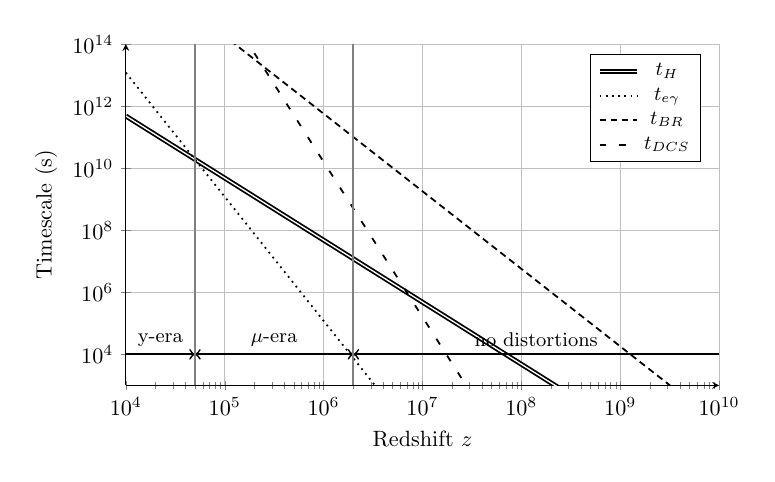
\begin{tikzpicture}[scale=.8]
            \begin{axis}[
                width=11cm, height=7cm,
                xlabel={Redshift $z$},
                ylabel={Timescale (s)},
                xmin=1e4, xmax=1e10,
                ymin=1e3, ymax=1e14,
                xmode=log,
                ymode=log,
                legend pos=north east,
                grid=major,
                axis lines=left,
                legend style={font=\small}
            ]
                % t_H (radiation domination)
                \addplot[
                    domain=1e4:1e10,
                    samples=200,
                    thick,
                    double
                ] {4.8e19 * (1 + x)^(-2)};
                \addlegendentry{$t_H$ }

                % t_{e\gamma}
                \addplot[
                    domain=1e4:1e10,
                    samples=200,
                    thick,
                    dotted
                ] {1.2e29 * (1 + x)^(-4)};
                \addlegendentry{$t_{e\gamma}$ }

                % t_{BR}
                \addplot[
                    domain=1e4:1e10,
                    samples=200,
                    thick,
                    densely dashed
                ] {1.9*3e26 *  (1 + x)^(-2.5)};
                \addlegendentry{$t_{\text{BR}}$ }

                % t_{DCS}
                \addplot[
                    domain=1e4:1e10,
                    samples=200,
                    thick,
                    loosely dashed
                ] {1.6e40 * (1 + x)^(-5)};
                \addlegendentry{$t_{\text{DCS}}$ }

                \draw[->, thick] (axis cs:1e4,1e4) -- (axis cs:5e4,1e4)
                    node[midway, above, font=\small] {y-era};
                \draw[<->, thick] (axis cs:5e4,1e4) -- (axis cs:2e6,1e4)
                    node[midway, above, font=\small] {$\mu$-era};
                \draw[<-, thick] (axis cs:2e6,1e4) -- (axis cs:1e10,1e4)
                    node[midway, above, font=\small] {no distortions};

                \draw[gray, thick] (axis cs:2e6,1e3) -- (axis cs:2e6,1e14);
                \draw[gray, thick] (axis cs:5e4,1e3) -- (axis cs:5e4,1e14);
            \end{axis}
        \end{tikzpicture}
        \caption{Timescales of relevant processes.}
        \label{fig:timescales_and_criticalfreq}
    \end{subfigure}
    \hfill
    % Second subfigure: Critical frequencies
    \begin{subfigure}[b]{0.48\textwidth}
        \centering
        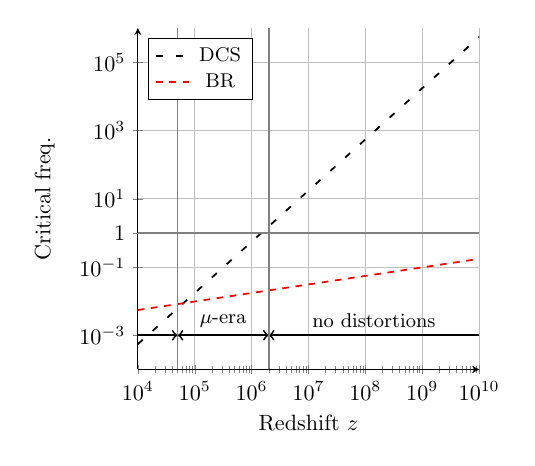
\begin{tikzpicture}[scale=.8]
            \begin{axis}[
                width=7cm, height=7cm,
                xlabel={Redshift $z$},
                ylabel={Critical freq.},
                xmin=1e4, xmax=1e10,
                ymin=1e-4, ymax=1e6,
                xmode=log,
                ymode=log,
                extra y ticks={1},
                extra y tick labels={$1$},
                legend pos=north west,
                grid=major,
                axis lines=left,
                legend style={font=\small}
            ]
                % x_crit, DCS
                \addplot[
                    domain=1e4:1e20,
                    samples=200,
                    thick,
                    loosely dashed
                ] {5.5e-10 * (1 + x)^(1.5)};
                \addlegendentry{ DCS}

                % x_crit, BR
                \addplot[
                    domain=1e4:1e20,
                    samples=200,
                    thick,
                    red,
                    dashed
                ] {5.5e-4 * (1 + x)^(0.25)};
                \addlegendentry{ BR}
                \draw[->, thick] (axis cs:1e4,1e-3) -- (axis cs:5e4,1e-3);
                \draw[<->, thick] (axis cs:5e4,1e-3) -- (axis cs:2e6,1e-3)
                    node[midway, above, font=\small] {$\mu$-era};
                \draw[<-, thick] (axis cs:2e6,1e-3) -- (axis cs:1e10,1e-3)
                    node[midway, above, font=\small] {no distortions};
                \draw[gray, thick] (axis cs:1e4,1) -- (axis cs:1e10,1) ;
                \draw[gray, thick] (axis cs:2e6,1e-4) -- (axis cs:2e6,1e14);
                \draw[gray, thick] (axis cs:5e4,1e-4) -- (axis cs:5e4,1e14);
            \end{axis}
        \end{tikzpicture}
        \caption{Maximum relevant freq.}
        \label{fig:critical_frequencies}
    \end{subfigure}
    \caption{Comparison of CS, BR and DCS with the expansion of the universe. Left: Timescale comparison: when each $t>t_H$ the process becomes inefficient. Right: Maximum frequencies at which DCS and BR are efficient as function of $z$.}
\end{figure}
As we discussed, also Bremsstrahlung and double Compton scatterings affect the thermalization of the photon plasma, mainly by changing the number of photons. First, by estimating the two factors in equations \eqref{eq:C_Bremsstrahlung} and \eqref{eq:C_DCS} (using quantities typical off $z>10^3$) as done by J. Chluba in \cite{chlubafuturestepscosmologyusing}
$$K_\text{BR}\approx1.4\times10^{-6}\bigg(\frac{\bar{g}_\text{ff}}{3.0}\bigg)\bigg(\frac{\Omega_b h^2}{0.022}\bigg)(1+z)^{-1/2}\quad\text{and }K_\text{DCS}\approx1.7\times10^{-20}(1+z)^2,$$ we discover that at higher redshift is the double Compton scattering to dominate over Bremsstrahlung. Then, to understand when these interactions are relevant we can compare their timescales to $t_H$: for low frequency photons we have
\begin{align*}
    t_{\text{BR}}&=\frac{t_Te^{x}x^3}{K_\text{BR}(1-e^{x_e})}\approx1.9\times10^{26}\bigg(\frac{\bar{g}_{ff}}{3}\bigg)^{-1}\bigg(\frac{\Omega_bh^2}{0.022}\bigg)^{-1}(1+z)^{-5/2}s,\\
    t_{\text{DCS}}&=\frac{t_Te^{2x}x^3}{K_\text{DCS}(1-e^{x_e})}\approx1.6\times10^{40}(1+z)^{-5}.
\end{align*}
Note that the timescales of these processes are also determined by the frequency $x_e$ and $x$ of the photons: in general these are efficient at high redshifts or for low frequency photons. The comparison of these timescales with $t_H$ allows us to obtain the \emph{critical frequency} for which these are efficient at a given redshift: in the limit $x\ll1$ and assuming $T_z\approx T_e$ we find
\begin{align*}
    \text{DCS efficient for }x&>x_{\text{crit,DCS}}\defeq5.5\times10^{-10}(1+z)^{3/2}\\
    \text{BR efficient for }x&>x_{\text{crit,BR}}\defeq5.5\times10^{-4}(1+z)^{1/4}.
\end{align*}  
Overall, as shown in figure \ref{fig:critical_frequencies} for $z_{\text{th}}\approx2\times10^6$ both Bremsstrahlung and double Compton scattering become subdominant for high energy photons.

To proceed we should have in mind the following picture
\begin{enumerate}
    \item For $z>z_{\text{th}}\approx2\times10^6$ all the discussed interactions are efficient and thus, as we argued in the previous section, the plasma can fully thermalize to a blackbody radiation.
    \item For $z_{\text{th}}\approx2\times10^6>z>z_{\mu y}\approx 5\times 10^4$ Bremsstrahlung and double Compton scattering become subdominant, with respect to effect of the expansion of the universe on the photon plasma. Compton scattering is still efficient and thus photons and electrons can exchange energy, but the number of the former is almost fixed. This results in the possibility of generating \emph{spectral distortions} since, as we showed previously, Compton scattering thermalizes with a non-zero chemical potential. This range of redshifts is called $\boldsymbol{\mu}$\textbf{-era}.
    \item For $z>z_{\mu y}\approx 5\times 10^4$ also Compton scattering becomes inefficient and therefore obtaining a perfect blackbody spectrum through thermalization becomes even harder. The impossibility of fully reach equilibrium, in this period called \textbf{y-era}, can give rise to another type of spectral distortions.
\end{enumerate}
In the next sections we will focus on what kind of spectral distortions can be generated in these three phases and how they are generated.
\section{Modeling spectral distortions}
As we saw, at high redshifts the photon plasma will always thermalize to a blackbody radiation, which is in agreement with the observed CMB spectrum that turns out to be almost perfectly Planckian. Hence, spectral distortions will arise from deviations $\Delta f(x,t)$ from the \emph{Planckian blackbody} phase space distribution $B(x)\defeq(e^x-1)^{-1}$, as$$f(t,x)=B(x)+\Delta f(t,x),$$ where $x=\nu/(k_BT_z)$ as before. Then, every contribution $\Delta f(x,t)$ will also distort the \textbf{intensity spectrum} $$\mathcal{I}(t,x)=2(k_BT_z)^3 x^3f(t,x)=2(k_BT_z)^3[x^3B(x)+x^3\Delta f(t,x)],$$ which measures the energy of the radiation per unit frequency. Every distortion can then be further decomposed into a shape and an amplitude: the former one is determined by the physical process that generates the distortion while the latter measures how much the spectrum is distorted.

In the following sections we will study the distortions of the phase space distribution since the corresponding spectral distortions are obtained just by multiplying the former by $2(k_BT_z)^3x^3$.
\subsection{Shapes of spectral distortions}\label{sec:SD_shapes}
To determine the precise shape of the spectral distortions $\Delta f$ we must consider some energy injection in the plasma (in section \ref{sec:SD_injected_deposited_energy} we will discuss the nature of these injections) that perturbed equilibrium. We know that at different redshifts photons can thermalize in different ways since different interactions are efficient. 
\subsubsection{Temperature shift G}
At $z>z_\text{th}\approx2\times10^6$ photons can fully thermalize again to a blackbody spectrum, this means that after some energy is injected, a blackbody spectrum will be recovered but the injected energy will increase its temperature. Suppose that initially the plasma is at some temperature $T_z$, then, after the injection, the new temperature $T_z+\Delta T$ is reached: in this way, the distortion can be characterized by Taylor expanding for small $\Delta T$ the new phase space distribution 
$$B\bigg(\frac{\nu}{k_B(T_z+\Delta T)}\bigg)=B\bigg(\frac{x}{1+\Delta T/T_z}\bigg)\approx B(x)-x\frac{\partial B(x)}{\partial x}\frac{\Delta T}{T_z}\defeq B(x)+G(x)\frac{\Delta T}{T_z}.$$
From the above we recognize the shape of the distortion $G(x)$ and its amplitude $\Delta T/T_z$. The spectral distortion that we obtained is called \textbf{temperature shift}
\begin{equation}
    \label{eq:SD_temperature_shift}
    G(x)\defeq-x\frac{\partial B(x)}{\partial x}=\frac{xe^x}{(e^x-1)^2}.
\end{equation}
Note that, since $T_z$ is defined with respect to a reference temperature observed today $T_0$, it is always possible to readjust $T_0$ such that it coincides with the perturbed temperature today, in this way the temperature shift becomes essentially unobservable. 
\subsubsection{Chemical potential $\boldsymbol\mu$ distortion}
For $z_\text{th}>z>z_{\mu y}$ Bremsstrahlung and double Compton scattering are inefficient, thus the number of photons is almost fixed and only their energy can be redistributed through Compton scatterings. We already showed that from Kompaneets equation follows that a Bose-Einstein distribution with a non-zero chemical potential\footnote{Note that in the following the chemical potential uses the convection $f(x,\mu)=(e^{x+\mu}-1)^{-1}$ which is different from the usual definition by a factor $-1/(k_BT)$.} is reached at equilibrium (section \ref{sec:ThermalizationProblem}). This new phase space distribution, in the limit of $\mu/x\ll1$, can be reduced to deviation from the blackbody behavior using a Taylor expansion
$$f(x)=B(x+\mu)=(e^{x+\mu}-1)^{-1}\approx B(x)+\frac{\partial B(x)}{\partial x}\mu=B(x)-\mu\frac{G(x)}{x},$$
which suggests that the shape of the so-called $\boldsymbol\mu$\textbf{-distortion} should be $-G/x$ while its amplitude should be $\mu$. However, a simple calculation can show that such distortion would also result in a change of the number of photons from the initial one, since $\int d^3p B(x)$ is the initial number density of photons and
$$\int_0^\infty dx \frac{G(x)}{x}x^2=\int_0^\infty dx \frac{x^2e^x}{(e^x-1)^2}=2\zeta(2)\neq0,$$
while we know that in the $\mu$-era no extra photon is produced or destroyed.\\ 
We can remove this undesired behavior considering also a temperature shift: this extra distortion allows us to adjust the final number density of photons to be fixed.
\begin{align}
    \label{eq:SD_mu}
    &\qquad\qquad\qquad\qquad\qquad\qquad M(x)\defeq-G(x)\bigg(\frac{1}{x}-\alpha_\mu\bigg)\\
    0&=\int_0^\infty dx\ x^2M(x)=\int_0^\infty dx\ (-x^2+\alpha_\mu x^3)\frac{e^x}{(e^x-1)^2}=\int_0^\infty dx\ (x^2-\alpha_\mu x^3)\frac{d}{dx}\frac{1}{e^x-1}\nonumber\\&=\int_0^\infty dx\ (-2x+\alpha_\mu 3x^2)\frac{1}{e^x-1}=\sum_{k=0}^{\infty}\int_0^\infty dx\ (-2x+\alpha_\mu 3x^2)e^{-x(k+1)}\nonumber\\&=\sum_{k=0}^{\infty}\bigg(-\frac{2}{(k+1)^2}+\alpha_\mu\frac{6}{(k+1)^3}\bigg)=-2\zeta(2)+6\alpha_\mu\zeta(3)\nonumber\\
    &\qquad\qquad\qquad\quad\qquad\qquad\Longrightarrow\alpha_\mu=\frac{\zeta(2)}{3\zeta(3)}\approx0.4561.\nonumber
\end{align}
With this correction we finally have that a $\boldsymbol\mu$\textbf{-disortion} is given by$$\Delta f(x)=\mu M(x)\defeq-\mu G(x)\bigg(\frac{1}{x}-0.4561\bigg).$$

\subsubsection{Compton y distortion}
Lastly, for $z<z_{\mu y}$ also energy transfer by Compton scattering becomes inefficient, this means that equilibrium is never fully reached after some energy injection, for example. In this case we can obtain a shape for the spectral distortions by exploiting the Kompaneets equation \eqref{eq:C_compton}
$$\frac{\partial f}{\partial t}=n_e\sigma_T\frac{k_BT_e}{m_e}x^{-2}\frac{\partial}{\partial x}\bigg[x^4\bigg(\frac{\partial f}{\partial x}+\frac{T_z}{T_e}f(1+f)\bigg)\bigg].$$ Recall that in the above we exploited the time independence of $x$ to rewrite $\hat{L}[f]=\frac{\partial f}{\partial t}.$
Considering an initial blackbody distribution $B(x)$, this equation gives us an estimate for the change of phase space distribution over a small lapse of time $\Delta t$ $$\Delta f\approx n_e\sigma_T\frac{k_BT_e}{m_e}x^{-2}\frac{\partial}{\partial x}\bigg[x^4\bigg(\frac{\partial B(x)}{\partial x}+\frac{T_z}{T_e}B(x)(1+B(x))\bigg)\bigg]\Delta t.$$
Some simple algebra can show that $-\frac{\partial B}{\partial x}=B(x)(1+B(x))=\frac{G(x)}{x}=\frac{e^x}{(e^x-1)^2}$, so that the above reads in the end
\begin{equation}
    \label{eq:SD_y_distortion}
    \Delta f=yY(x)\defeq -y\frac{1}{x^2}\frac{\partial}{\partial x}\bigg(x^3G(x)\bigg)=y\ G(x)\bigg(x\frac{e^x+1}{e^x-1}-4\bigg),
\end{equation}
where $Y$ is the shape of the so-called \textbf{y-distortion} and $y=n_e\sigma_Tk_B\frac{T_e-T_z}{m_e}\Delta t$ is its amplitude. Observe that this distortion already conserves the number density of photons, since
$$\int_0^\infty dx\ x^2Y(x)=\int_0^\infty dx\ x^2G(x)\bigg(x\frac{e^x+1}{e^x-1}-4\bigg)=0,$$
and therefore no extra temperature shift is needed this time.

Note that an inefficient Compton scattering interaction is not the only way to generate a y-distortion. Indeed, by Taylor expanding at second order in $\Delta T/T_z$ a temperature shift we can produce a distortion with the same shape as a y-distortion.
\begin{align}
    \nonumber B\bigg(\frac{x}{1+\Delta T/T_z}\bigg)&\approx B(x)+\frac{\partial}{\partial \frac{\Delta T}{T_z}}\bigg(e^{\frac{x}{1+\Delta T/T_z}}-1\bigg)^{-1}\frac{\Delta T}{T_z}+\frac{1}{2}\frac{\partial^2}{\partial \frac{\Delta T}{T_z}^2}\bigg(e^{\frac{x}{1+\Delta T/T_z}}-1\bigg)^{-1}\bigg(\frac{\Delta T}{T_z}\bigg)^2\\&\nonumber\approx B(x)+x\frac{e^x}{(e^x-1)^2}\frac{\Delta T}{T_z}-\frac{1}{2}\frac{e^xx}{(e^x-1)^2}\bigg[x-\frac{2e^{x}}{e^x-1}+2\bigg]\bigg(\frac{\Delta T}{T_z}\bigg)^2\\ \nonumber&= B(x)+G(x)\frac{\Delta T}{T_z}-\frac{1}{2}\frac{xe^x}{(e^x-1)^2}\bigg[\frac{x(e^x-1)-2xe^x}{e^x-1}-2\bigg]\bigg(\frac{\Delta T}{T_z}\bigg)^2\\&=B(x)+G(x)\frac{\Delta T}{T_z}+\frac{1}{2}[Y(x)+2G(x)]\bigg(\frac{\Delta T}{T_z}\bigg)^2.\label{eq:SD_2ord_temp_shift}
\end{align}
We can see that, overall, a temperature shift of amplitude $\Delta T/T_z+(\Delta T/T_z)^2$ and a y-distortion of amplitude $1/2\times(\Delta T/T_z)^2$ are generated. This could seem like some trivia: instead one of the main mechanism that we will study in the next sections will rely on the necessity to expand a temperature shift up to the second order, generating this distortion.
\begin{figure}[h]
\begin{multicols}{2}
    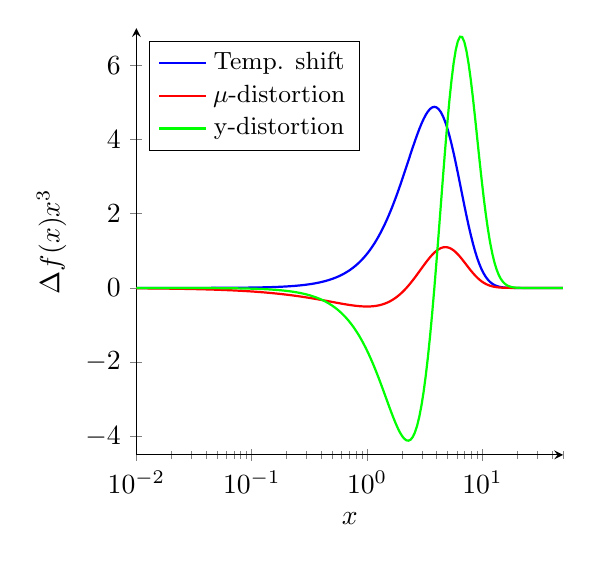
\begin{tikzpicture}
        \begin{axis}[
            width=7cm, height=7cm,
            xlabel={$x$}, ylabel={$\Delta f(x)x^3$},
            xmin=0.01, xmax=50, % Avoid x=0 to prevent division by zero
            ymin=-4.5, ymax=7, xmode=log,
            restrict y to domain=-4.5:7, % Restrict y-values to avoid extreme values
            legend pos=north west,
            axis lines=left,
            legend style={font=\small}
        ]
            % Plot for G(x) = x * exp(x) / (exp(x) - 1)^2
            \addplot[
                domain=0.01:50, % Avoid x=0 to prevent division by zero
                samples=200,
                thick,
                blue
            ] {(x^4 * exp(x) / (exp(x) - 1)^2)};
            \addlegendentry{Temp. shift}

            % Plot for M(x) = -G(x) * (1/x - 0.4561)
            \addplot[
                domain=0.01:50,
                samples=200,
                thick,
                red
            ] {-x^3*(x * exp(x) / (exp(x) - 1)^2) * (1/x - 0.4561)};
            \addlegendentry{$\mu$-distortion}

            % Plot for Y(x) = G(x) * (x * (exp(x)+1)/(exp(x)-1) - 4)
            \addplot[
                domain=0.01:50,
                samples=200,
                thick,
                green
            ] {x^3*(x * exp(x) / (exp(x) - 1)^2) * (x * (exp(x) + 1) / (exp(x) - 1) - 4)};
            \addlegendentry{y-distortion}
        \end{axis}
    \end{tikzpicture}

    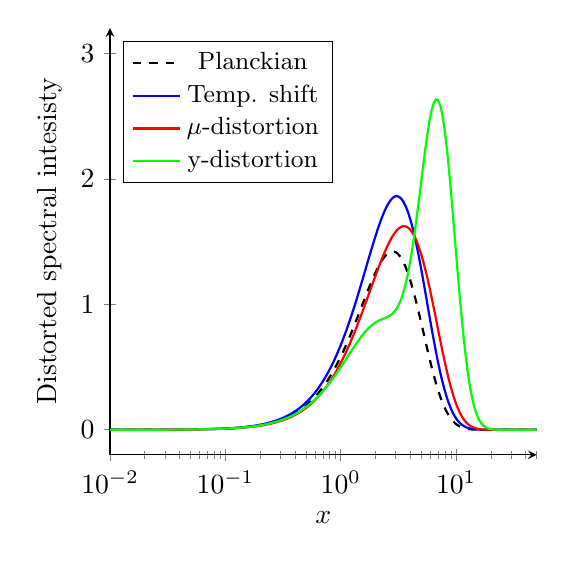
\begin{tikzpicture}
        \begin{axis}[
            width=7cm, height=7cm,
            xlabel={$x$}, ylabel={Distorted spectral intesisty},
            xmin=0.01, xmax=50, % Avoid x=0 to prevent division by zero
            ymin=-.2, ymax=3.2, xmode=log,
            restrict y to domain=-0.2:3.2, % Restrict y-values to avoid extreme values
            legend pos=north west,
            axis lines=left,
            legend style={font=\small}
        ]
            % Planckian blackbody spectrum B(x) * x^2
            \addplot[
                domain=0.01:50,
                samples=200,
                thick,
                black,
                dashed
            ] {x^3 / (exp(x) - 1)};
            \addlegendentry{Planckian }

            % Temp. shift G(x) + Planckian
            \addplot[
                domain=0.01:50,
                samples=200,
                thick,
                blue
            ] {(x^3 / (exp(x) - 1)) + .1*(x^4 * exp(x) / (exp(x) - 1)^2)};
            \addlegendentry{Temp. shift }

            % $\mu$-distortion M(x) + Planckian
            \addplot[
                domain=0.01:50,
                samples=200,
                thick,
                red
            ] {(x^3 / (exp(x) - 1)) - .1*(x^4 * (x * exp(x) / (exp(x) - 1)^2) * (1/x - 0.4561))};
            \addlegendentry{$\mu$-distortion }

            % y-distortion Y(x) + Planckian
            \addplot[
                domain=0.01:50,
                samples=200,
                thick,
                green
            ] {(x^3 / (exp(x) - 1)) +.05 *(x^4 * (x * exp(x) / (exp(x) - 1)^2) * (x * (exp(x) + 1) / (exp(x) - 1) - 4))};
            \addlegendentry{y-distortion }
        \end{axis}
    \end{tikzpicture}
\end{multicols}
\caption{Shapes of the spectral distortions plotted by their spectral intensity $\mathcal{I}\propto f(x)x^3$. The plot on the left shows the three spectral distortions with unitary amplitudes. The plot on the right compares the Planckian spectrum and the three distorted ones (Planckian + distortion).}
\label{fig:SD_shapes}
\end{figure}

\subsubsection{Residual distortion}
A more refined discussion should also consider non-thermal processes, such as atomic transitions, that could generate spectral distortions. Since these processes are less relevant for our purpose, but they still contribute to the full energy balance of spectral distortions, we will define the \textbf{residual distortion} $R(x)$ that will account for those. In the end numerical methods will allow also to determine this distortion.
\subsection{Amplitudes of spectral distortions}\label{sec:SD_amplitudes}
Now that we know which are the shapes of the of spectral distortions that we expect to observe in the \emph{CMB}, we want to understand how their respective amplitudes can be obtained and what is their meaning.

In the previous section we derived the form of the different amplitudes as functions of temperatures or of the chemical potential. However, when studying the effects of energy injections in the plasma, it is useful to relate the amplitudes to the injected energy. This can easily be accomplished by considering that the energy density contribution of each spectral distortion must correspond to the injected energy that generated them in the first place. In this way, recalling that $\rho=\int d^3pf(p,t)E=4\pi (k_BT_z)^4\int dxf(x)x^3$ since $E=p=\nu$ and $x=\nu/(k_BT_z)$, we can write
\begin{align}
    \label{eq:SD_g_amplitude}\frac{\Delta \rho_\gamma}{\rho_\gamma}\bigg|_g&=g\frac{\int dxG(x)x^3}{\int dx B(x)x^3}=4g\quad\Rightarrow\quad &\boxed{g=\frac{1}{4}\frac{\Delta \rho_\gamma}{\rho_\gamma}\bigg|_g}\quad \text{Temp. Shift,}\\\label{eq:SD_mu_amplitude}
    \frac{\Delta \rho_\gamma}{\rho_\gamma}\bigg|_\mu&=\mu\frac{\int dxM(x)x^3}{\int dx B(x)x^3}=\frac{\mu}{1.401}\quad\Rightarrow\quad &\boxed{\mu=1.401\frac{\Delta \rho_\gamma}{\rho_\gamma}\bigg|_\mu}\quad\mu\text{-distortion,}\\\label{eq:SD_y_amplitude}
    \frac{\Delta \rho_\gamma}{\rho_\gamma}\bigg|_y&=y\frac{\int dxY(x)x^3}{\int dx B(x)x^3}=4y\quad\Rightarrow\quad &\boxed{y=\frac{1}{4}\frac{\Delta \rho_\gamma}{\rho_\gamma}\bigg|_y}\quad\text{y-distortion.}
\end{align}


Let's stop for a while to appreciate the physical meaning of each of these amplitudes. Indeed, in the above, we could even consider energy extraction from the plasma, therefore some physical considerations are needed. From our discussion on the shapes it is already clear that $g$ is just a measure of the change of temperature of the blackbody radiation (equation \eqref{eq:SD_temperature_shift}), in this way some energy extraction would correspond to a decrease of the temperature ($g<0$). In the same way  $\mu$, from equation \eqref{eq:SD_mu}, is the chemical potential: physically its appearance means that the photon plasma hasn't the same number of particle that a blackbody radiation at the same temperature would have. In particular, since the chemical potential measures the energy necessary to change the number of particles:
\begin{itemize}
    \item $\mu>0$ distortions are generated by an energy injection, since we now have \emph{more energetic but fewer photons} compared to a blackbody radiation at the same temperature;
    \item $\mu<0$ is the result of an energy extraction that just lowered the energy of each photon leaving \emph{more photons} than the corresponding blackbody radiation.
\end{itemize}
Lastly, considering that a y-distortion is produced when thermalization is not completely reached, we can distinguish between $y>0$, when some energy is still being (inefficiently) transferred from electrons to photons, and $y<0$, when the opposite occurs. In the former case, scatterings cause \emph{Comptonization}, while in the latter they cause \emph{Compton cooling}. 

Usually only energy injections will occur in the early universe, as most of the processes tend to heat the plasma. For the purpose of this work energy extractions will be considered negligible and only positive amplitudes will be allowed.  
\subsection{Injected, deposited energy and heating rate}\label{sec:SD_injected_deposited_energy}
In the previous sections we argued that spectral distortions are generated by injection of energy in the photon plasma when some scattering process has become inefficient. However, this description is still not accurate enough: indeed, after the injection, the energy can be subject to other processes (e.g. adiabatic cooling due to the expansion of the universe or production of non-interacting particles) that can change the amount energy that generates spectral distortions. 

To refine our description of the injected energy, we must differentiate between \textbf{injected energy} and \textbf{deposited energy}. The former is the energy that a certain process transfer to the plasma, while the latter is the energy that heats the plasma and contributes to the spectral distortions.\\ For each process that injects energy in the channel $c$ (which describes the form of the heat), we define the \textbf{deposition function} $f_c(z)$. This function describes, at a given redshift, the fraction of injected energy that is deposited in the plasma. We can further decompose this function into an \textbf{injection efficiency function } $f_{\text{eff}}(z)$ and a \textbf{deposition fraction} $\chi_{c}(z)$. The former describes how much energy is deposited regardless the form and depends on the injecting process and on the universe conditions, while the latter accounts for the fraction deposited in each channel, with $\sum_c\chi_c=1$. Overall we have
\begin{equation}\label{eq:deposition_function}
    \frac{dE}{dt dV}\bigg|_{\text{dep},c}=\frac{dE}{dt dV}\bigg|_{\text{inj}}f_c(z)=\frac{dE}{dt dV}\bigg|_{\text{inj}}f_{\text{eff}}(z)\chi_c(z)\defeq \dot{\mathcal{Q}}(z)\chi_c(z).
\end{equation}
To understand the meaning of this decomposition consider a process that injects energy in the form of different kinds of particles. If some species do not interact electromagnetically (for example neutrinos) they will not be able to exploit Comptonization to transfer energy to the photon plasma: the injection efficiency function will account for this.

Furthermore, the injection efficiency does not correspond to the energy transferred by electromagnetic interactions. Indeed, as it happens during the Dark ages, when the scattering rate is too low to thermalize the plasma immediately, some injected energy is lost due to the adiabatic cooling caused by the expansion of the universe. However, at pre-recombinatory redshifts, scatterings are frequent enough to thermalize the plasma almost immediately. In this case it is usually employed the so-called \emph{on-the-spot} approximation, for which no energy is lost due to a non-istantaneous deposition. For our purposes, since we will always consider high redshifts (as explained in section \ref{sec:ThermalizationScales}), we will always use this approximation.

Lastly, we should account for the possibility of heating the photon component of the plasma by energy transfers among the different species or even by some energy redistribution among the photons themselves. This can happen, for example, during adiabatic cooling of different species: different cooling rates results in energy transfers between the species to reestablish equilibrium.   In this case no energy is injected but in the end spectral distortions can still be generated. To describe this last effect we define the \textbf{non-injected heating rate} $\dot{Q}_\text{non-inj}$, so that the heating rate of the photon plasma reads
\begin{equation}
    \dot{Q}=\frac{dE}{dtdV}\bigg|_{\text{dep,c}}+\dot{Q}_\text{non-inj}=\dot{\mathcal{Q}}(z)\chi_c+\dot{Q}_\text{non-inj}.\label{eq:heating_rate}
\end{equation}

Now that we have a full picture of how energy is injected in the plasma of photons, let's connect the heating rate to the spectral distortion amplitudes that we obtained in section \ref{sec:SD_amplitudes}. We can relate the heating rate to the energy density using the Liouville operator, starting from the definition of the energy density
\begin{align*}
    \rho = \int d^3p\ f(p,t)E\quad \Rightarrow\quad \dot{Q}&=\int d^3p\ \frac{df}{dt} E=\int_0^\infty 4\pi p^2dp\ \bigg(\frac{\partial f}{\partial t}-Hp\frac{\partial f}{\partial p}\bigg)p\\
    &=\frac{\partial \rho}{\partial t} -4\pi H\int_0^\infty  dp\ \frac{\partial f}{\partial p}p^4=\frac{\partial \rho}{\partial t} +16\pi H\int_0^\infty  dp\ f(p,t)p^3\\&=\frac{\partial \rho}{\partial t} +4H\rho=\frac{1}{a^4}\frac{\partial (a^4 \rho)}{\partial t},
\end{align*}
in this way we obtained a differential equation for $\rho$, for which $\dot{Q}$ is a source term
\begin{equation*}
    \frac{\partial (a^4 \rho)}{\partial t}=a^4\dot{Q}.
\end{equation*}
The general solution of this equation $\rho(t)$ is made of a homogeneous solution $\rho_z(t)$ and a particular solution $\Delta\rho(t)$. The homogeneous solution, obtained in absence of heating, is just the energy density of decoupled photons in the expanding universe $\rho_z\propto a^{-4}$. On the other hand, the particular solution $\Delta\rho(t)$ is the energy density deviation from the homogeneous one, that we related in section \ref{sec:SD_amplitudes} to the spectral distortion amplitudes. Upon integration, we find that the particular solution reads
$$\Delta\rho(t)=\frac{1}{a^4}\int dt'\ a^4\dot{Q}(t')=\rho_z\int dt'\ \frac{\dot{Q}(t')}{\rho_z}.$$
We can now find an explicit expression for the left and side of equations \eqref{eq:SD_g_amplitude}, \eqref{eq:SD_mu_amplitude} and \eqref{eq:SD_y_amplitude} by considering $\Delta\rho=\Delta\rho_\gamma$ and $\rho_\gamma=\rho_z$
\begin{equation}
    \frac{\Delta \rho_\gamma}{\rho_\gamma}=\int dt\frac{\dot Q}{\rho_\gamma}=\int dz\frac{\dot Q}{(1+z)H\rho_\gamma}=\int dz\frac{dQ/dz}{\rho_\gamma},\label{eq:SD_Deltarho_rho}
\end{equation}
where we used that $dz=-H(1+z)dt$.

Note that an alternative notation for the heating rate is sometimes used in the literature. Indeed, equation \eqref{eq:SD_Deltarho_rho} implies that $\dot Q/\rho_\gamma$ is (by the fundamental theorem of calculus) the time derivative of $\Delta\rho_\gamma/\rho_\gamma$. In this way, some papers refers to the heating rate as $\frac{d}{dt}\frac{\Delta \rho_\gamma}{\rho_\gamma}$. Hence, the two conventions are equivalent.
\subsection{Branching rations and the Green's function approach}
In the previous section we reduced the problem of determining the distortions in the CMB spectrum to the task of integrating the heating rate over time (equation \eqref{eq:SD_Deltarho_rho}). In section \ref{sec:ThermalizationScales} we showed that different types of distortions arise in different epochs of the universe since different interactions are efficient. Hence, when dealing with the heating rate we must take into account the thermal state of the universe. This can be accomplished by introducing the \textbf{branching rations} $\mathcal{J}_a(z)$: each of these functions describes the fraction of the deposited energy that contributes to a specific distortion $a$ at redshift $z$. In this way, using the equation \eqref{eq:SD_Deltarho_rho} with \eqref{eq:SD_g_amplitude}, \eqref{eq:SD_mu_amplitude} and \eqref{eq:SD_y_amplitude} that we just derived in the previous section, we get that a given amplitude $a$ can be evaluated as
\begin{equation}
    a=C_a\frac{\Delta\rho_\gamma}{\rho_\gamma}\bigg|_a=C_a\int dz\frac{dQ/dz}{\rho_\gamma}\mathcal{J}_a(z),\quad\text{for } a=g,\mu,y,\label{eq:SD_amplitude_branching},
\end{equation}
where $C_a$ is the constant that relates the amplitude of each distortion to the fraction of deposited energy, and they are $C_g=1/4$, $C_\mu=1.401$ and $C_y=1/4$.\\
This splits the general problem in two independent subproblems: determining the heating rate $d Q/dz$, which depends on the specific model that inject energy in the plasma, and solving for the branching ratios, which instead is independent of the injecting mechanism and is determined only by the thermal history of the universe.

Different approaches can be taken to obtain the branching ratios, we will now describe the main approximations and how to obtain the exact solution. From the discussion of section \ref{sec:ThermalizationScales} one could get a brute approximation for the branching ratios as step functions that allows for a certain distortion to be produced only during its specific era.
\begin{equation}
    \mathcal{J}_g(z)=\Theta_{H}(z-z_\text{th}),\quad \mathcal{J}_\mu(z)=\Theta_{H}(z_\text{th}-z)\Theta_{H}(z-z_{\mu y}),\quad \mathcal{J}_y(z)=\Theta_{H}(z_{\mu y}-z),
\end{equation}
with $z_\text{th}\approx2\times10^6$ and $z_{\mu y}\approx5\times10^4$.
In this way we are assuming that the transition from one era to another is instantaneous, which clearly is not the case. 

To improve this approximation we can consider that the chemical potential of the $\mu$-distortions is frequency dependent (some ref). This happens because, as we discussed in section \ref{sec:ThermalizationProblem}, for low energy photons these two processes can still be efficient even in the $\mu$-era. Studying the full Boltzmann equation (as in ref) we can find an approximate solution of the frequency dependence of the chemical potential 
\begin{equation*}
    \label{eq:SD_mu_freq}
    \mu(x,t)\approx\mu_0e^{-x_c(t)/x}e^{-(z/z_{\text{th}})^{5/2}},
\end{equation*}
where $x_c$ is the critical frequency and $z_{\text{th}}$ is the redshift at which the Compton scattering becomes inefficient. This suggests that the $\mu$ branching ratio can be approximated by $f(z)\defeq e^{-(z/z_{\text{th}})^{5/2}}$, giving in the end
\begin{equation}
    \mathcal{J}_g(z)=1-f(z),\quad \mathcal{J}_\mu(z)=f(z),\quad \mathcal{J}_y(z)=f(z)\Theta_{H}(z_{\mu y}-z),
\end{equation}
which describes a smooth $g$-$\mu$ transition and an instantaneous $\mu$-$ y$ transition.\\A further improvement is obtained by (ref 63 of lucca) considering a smooth $\mu$-$ y$ transition and results in the following branching ratios:
\begin{align}
    \mathcal{J}_g(z)&=1-f(z),\\ \mathcal{J}_\mu(z)&=f(z)\bigg\{1-\exp\bigg[-\bigg(\frac{1+z}{5.8\times10^4}\bigg)^{1.88}\bigg]\bigg\},\\\quad \mathcal{J}_y(z)&=\bigg[1+\bigg(\frac{1+z}{6\times10^{2.58}}\bigg)\bigg]^{-1}.
\end{align}
Note that in this last approximation the sum of all the branching ratios is not equal to one, this is due to the presence of the residual distortions we mentioned at the end of section \ref{sec:SD_shapes}. 

Finally, we can derive an exact solution for the branching ratios. This is done by exploiting \emph{Green's functions} methods to solve equation \eqref{eq:SD_Deltarho_rho}: we will now explain the main idea behind this method, but a more detailed explanation can be found in \cite{Lucca_2020}. To begin we consider the distorted spectral intensity associated with the photon plasma
$$\mathcal{I}(x,z)\defeq 2p^3f(p,t)=(k_BT_z)^3x^3\bigg[B(x)+G(x)+M(x)+Y(x)\bigg],$$
in which we used $x\defeq p/(k_BT_z)=\nu/(k_BT_z)$. Note that the intensity is the integrand function that gives the energy density of the plasma (upon integration over $p$ or equivalently $\nu$), and the factor $2$ accounts for the two polarization of the photons.
Now, the last three terms of the above are the spectral distortions, we thus define $\Delta \mathcal{I}$ as their sum.\\
We want to find the Green's function $G_{\text{th}}(x,z,z')$ that gives $\Delta \mathcal{I}(x,z)$ for an arbitrary heating rate as
$$\Delta \mathcal{I}(x,z)=\int dz'G_{\text{th}}(x,z,z')\frac{dQ(z')/dz'}{\rho_\gamma(z')}.$$
This has been done by J. Chluba \cite{Chluba_Green} by studying the full Boltzmann equation for photons and baryons. Then, a direct comparison with equation \eqref{eq:SD_amplitude_branching} relates the full Green's function to each branching rations
$$G_{\text{th}}(x,z=0,z')=\frac{1}{4}x^3G(x)\mathcal{J}_g(z')+1.401x^3M(x)\mathcal{J}_\mu(z')+\frac{1}{4}x^3Y(x)\mathcal{J}_y(z'),$$ in this way one can, from the full Green's function, obtain the branching ratios. Note that at this point a residual contribution can be added to obtain a measure of the residual distortion we introduced at the end of section \ref{sec:SD_shapes}.